% Chapter Template

\chapter{Diseño e Implementación} % Main chapter title

\label{Chapter3} % Change X to a consecutive number; for referencing this chapter elsewhere, use \ref{ChapterX}
En el siguiente capítulo se presentará el diseño y la implementación de las tres partes fundamentales del equipo. Se abarcarán aspectos de hardware, firmware, diseño y fabricación mecánica.
%----------------------------------------------------------------------------------------
%	SECTION 1
%----------------------------------------------------------------------------------------
\section{Hardware}
\subsection{Diseño basado en módulos de hardware libre}

Para la implementación del hardware se utilizó el software libre de diseño de circuitos impresos KICAD \citep{web_kicad}, que en sus últimas versiones presentá mejoras significativas respecto a sus predecesoras.

El diseño de la placa electrónica se baso en el estudio de los siguientes módulos:
\begin{itemize}
\item NodeMCU \citep{web_nodemcu}
\item TMC5130-EVAL \citep{3_web_trinamic_placa}	
\end{itemize}
Se destaca que ambos proyectos adhieren a la filosofía del hardware libre por lo tanto se pudieron descargar y estudiar los diagramas esquemáticos de ambas placas. 

El módulo TMC5130-EVAL como se describió en la sección \ref{sec:Circuitos integrados Trinamic} contiene al CI TMC5130. Del estudio de esta placa de evaluación se extrajeron las configuraciones necesarias para lograr la correcta utilización del driver. Se tuvieron en cuenta las recomendaciones de diseño establecidas por el fabricante como por ejemplo la incorporación de un clock externo de 16 MHz como se observa en la figura \ref{fig:kicad_clock} el cual es necesario en aplicaciones de alta precisión. 

\begin{figure}[h]
	\centering
	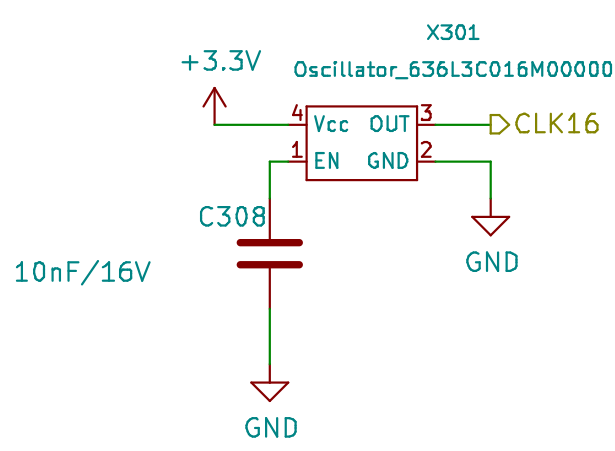
\includegraphics[width=.5\textwidth]{./Figures/kicad_clock.png}
	\caption{Clock para el CI TMC5130.}
	\label{fig:kicad_clock}
\end{figure}

Otra etapa importante como se observa en la figura \ref{fig:kicad_tension} es el regulador de tensión que permite alimentar al equipo con tensiones continuas entre 24 V y 46 V.
El equipo se diseño para ser alimentado con una fuente de alimentación externa simplificando así cuestiones regulatorias de certificación que deben cumplir equipos que se alimentan directamente con 220 V de tensión alterna.

\begin{figure}[h]
	\centering
	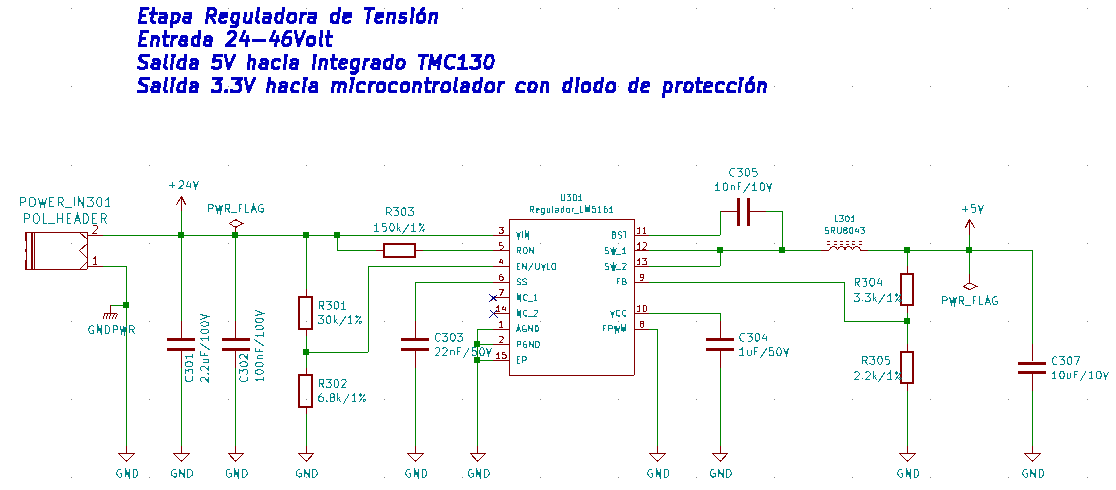
\includegraphics[width=1\textwidth]{./Figures/kicad_tension.png}
	\caption{Módulo de entrada.}
	\label{fig:kicad_tension}
\end{figure}
 
A continuación observamos en la figura \ref{fig:kicad_trinamic} las conexiones del driver con el motor paso a pasos y el puerto SPI utilizado para la comunicación con el microcontrolador. 
 
\begin{figure}[h]
	\centering
	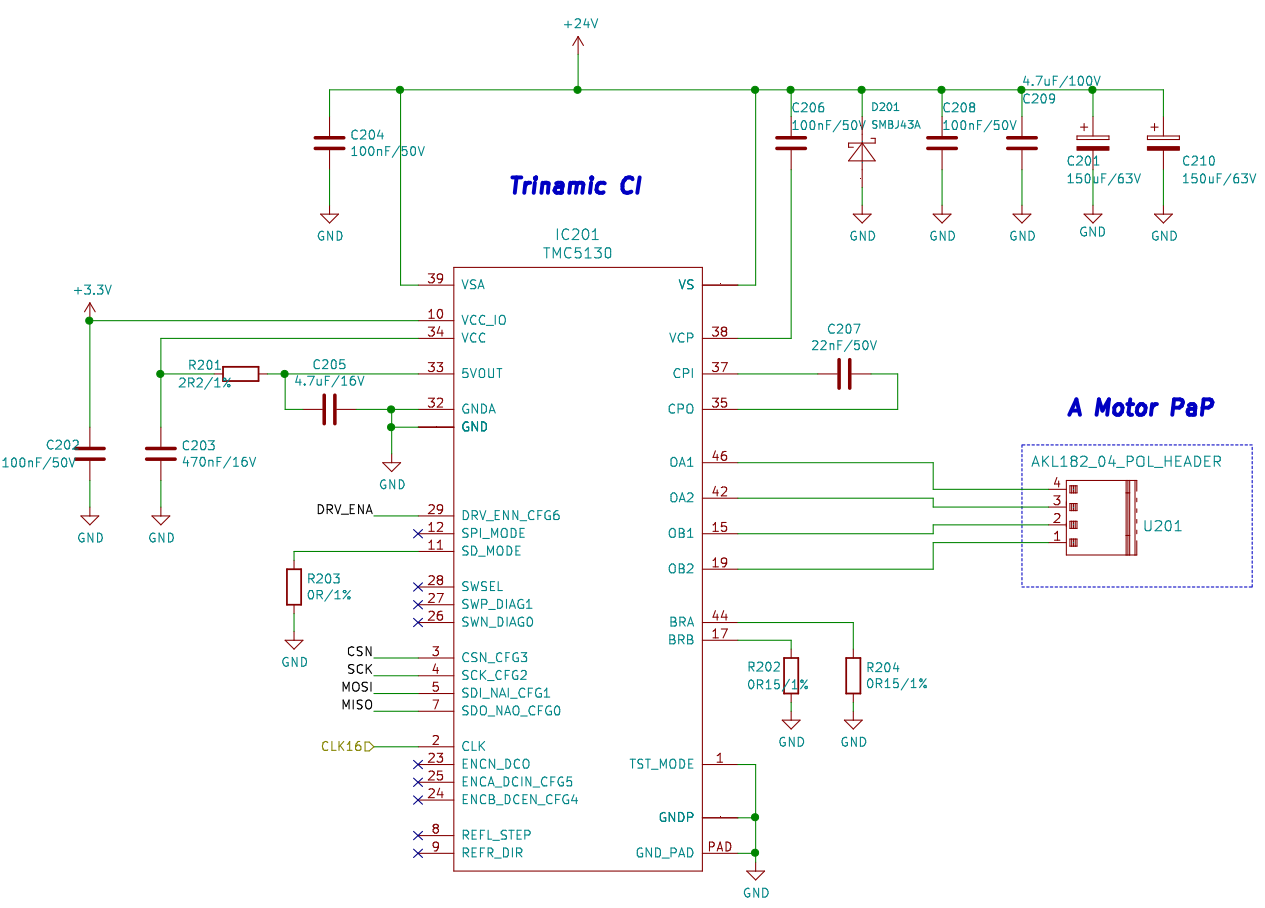
\includegraphics[width=1\textwidth]{./Figures/kicad_trinamic.png}
	\caption{CI TMC5130.}
	\label{fig:kicad_trinamic}
\end{figure} 
 
El cuanto al módulo NodeMCU es una placa de desarrollo que contiene el SoC ESP32-WROOM, del estudio de su diseño se implementó la etapa del conversor SERIAL-USB como se observa en la figura \ref{fig:kicad_conversor} que permite conectar el módulo directamente a un puerto USB de computadora para descargar el firmware y establecer una comunicación a través del periférico UART. Esto nos evita tener que contar con un programador externo.
\begin{figure}[h]
	\centering
	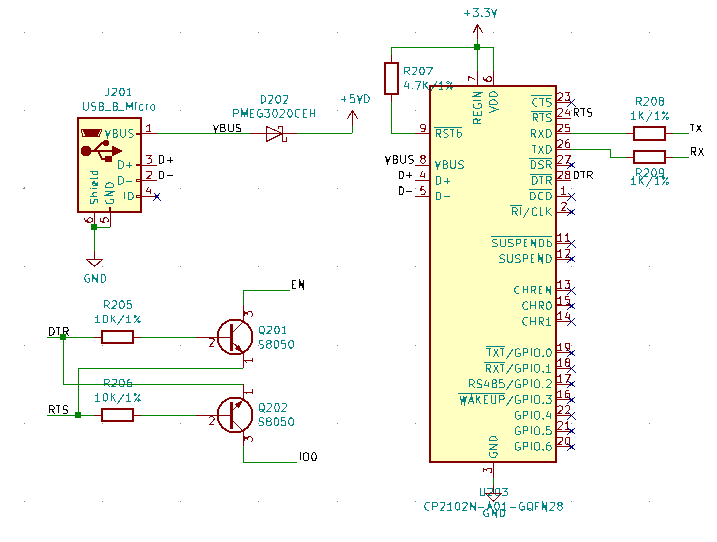
\includegraphics[width=1\textwidth]{./Figures/kicad_conversor.png}
	\caption{Conversor UART-USB.}
	\label{fig:kicad_conversor}
\end{figure}

%\begin{figure}[h]
%	\centering
%	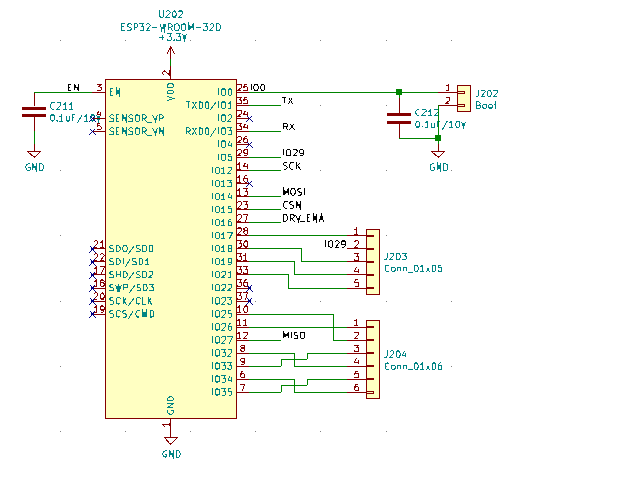
\includegraphics[width=.6\textwidth]{./Figures/kicad_esp.png}
%	\caption{Módulo ESP32.}
%	\label{fig:kicad_esp}
%\end{figure}
  
Finalmente podemos observar en la figura \ref{fig:dip_3d_model} el diseño 3D generado por el software KICAD cuyo diseño esta disponible en los repositorios de la empresa TECSCI \citep{web_hardware_tecsci}. La placa electrónica de este equipo dip coater cuenta con licencia CERN OHL v.1.2 \citep{web_cern_licence}.


\begin{figure}[h]
	\centering
	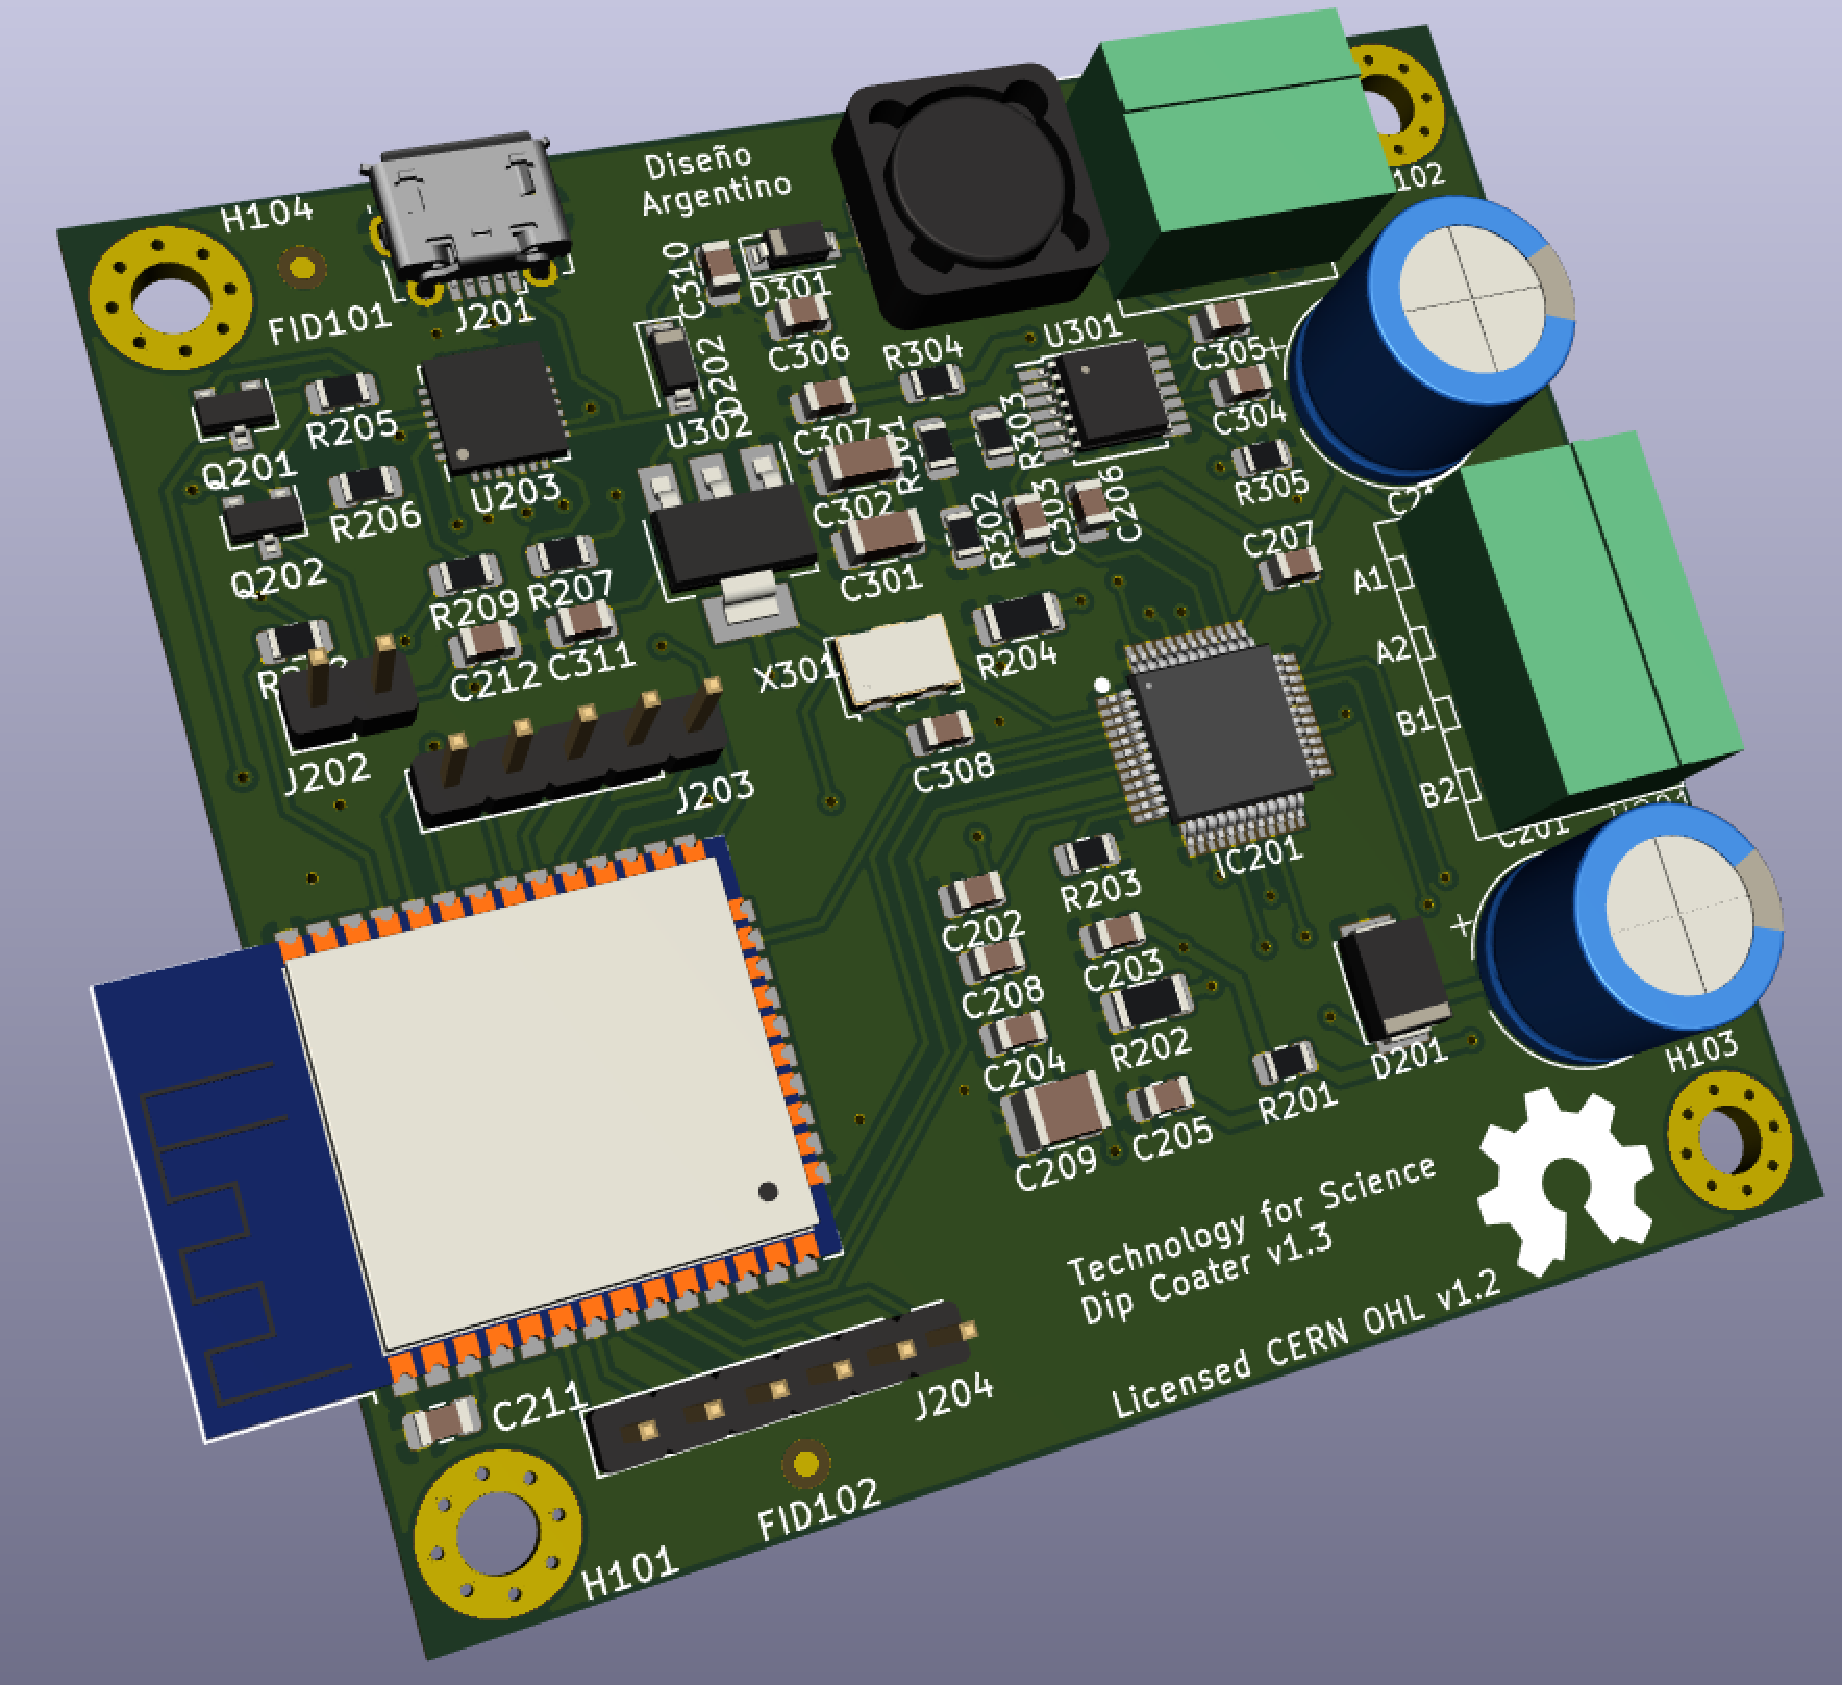
\includegraphics[width=.5\textwidth]{./Figures/dip_3d_model.pdf}
	\caption{Modelo 3D Kicad.}
	\label{fig:dip_3d_model}
\end{figure}
         



  
%-----------------------------------
%	SUBSECTION 1
%-----------------------------------
\subsection{Fabricación}
%-----------------------------------
%	SUBSECTION 2
%-----------------------------------
La placa electrónica se fabricó con el proveedor local de circuitos impresos Ernesto Mayer S.A. \citep{web_mayer}. A continuación se presenta la información de diseño de la placa y de describen algunas  restricciones de diseños impuestas por el fabricante:

\begin{itemize}

\item Grilla de posicionamiento principal: 0.25mm
\item Grilla de ruteo principal: 0.25mm
\item Agujeros de montaje: 3.2mm
\item Pistas principales: 0.5mm
\item Pistas inferiores: 0.25mm (límite particular 8mils(0.20mm))
\item Pistas superiores: 0.8mm
\item Vías: 0.8mm/0.4mm (límite particular 8mils(0.20mm))
\item Margen general: 0.22 mm
\item Margen particular: 0.2 mm (límite particual 8 mils(0.20mm))
\item Fabricación: espesor 1.6mm FR4  
\item Restricciones generales del fabricante: estándar 10 mils

\end{itemize}

Luego de fabricar el PCB, se continuó con el montaje de componentes electrónicos superficiales que estuvo a cargo de la empresa Asembli S.A. \citep{web_asembli}. Se fabricó un primer lote de cinco placas.


\begin{figure}[htbp]
	\centering
	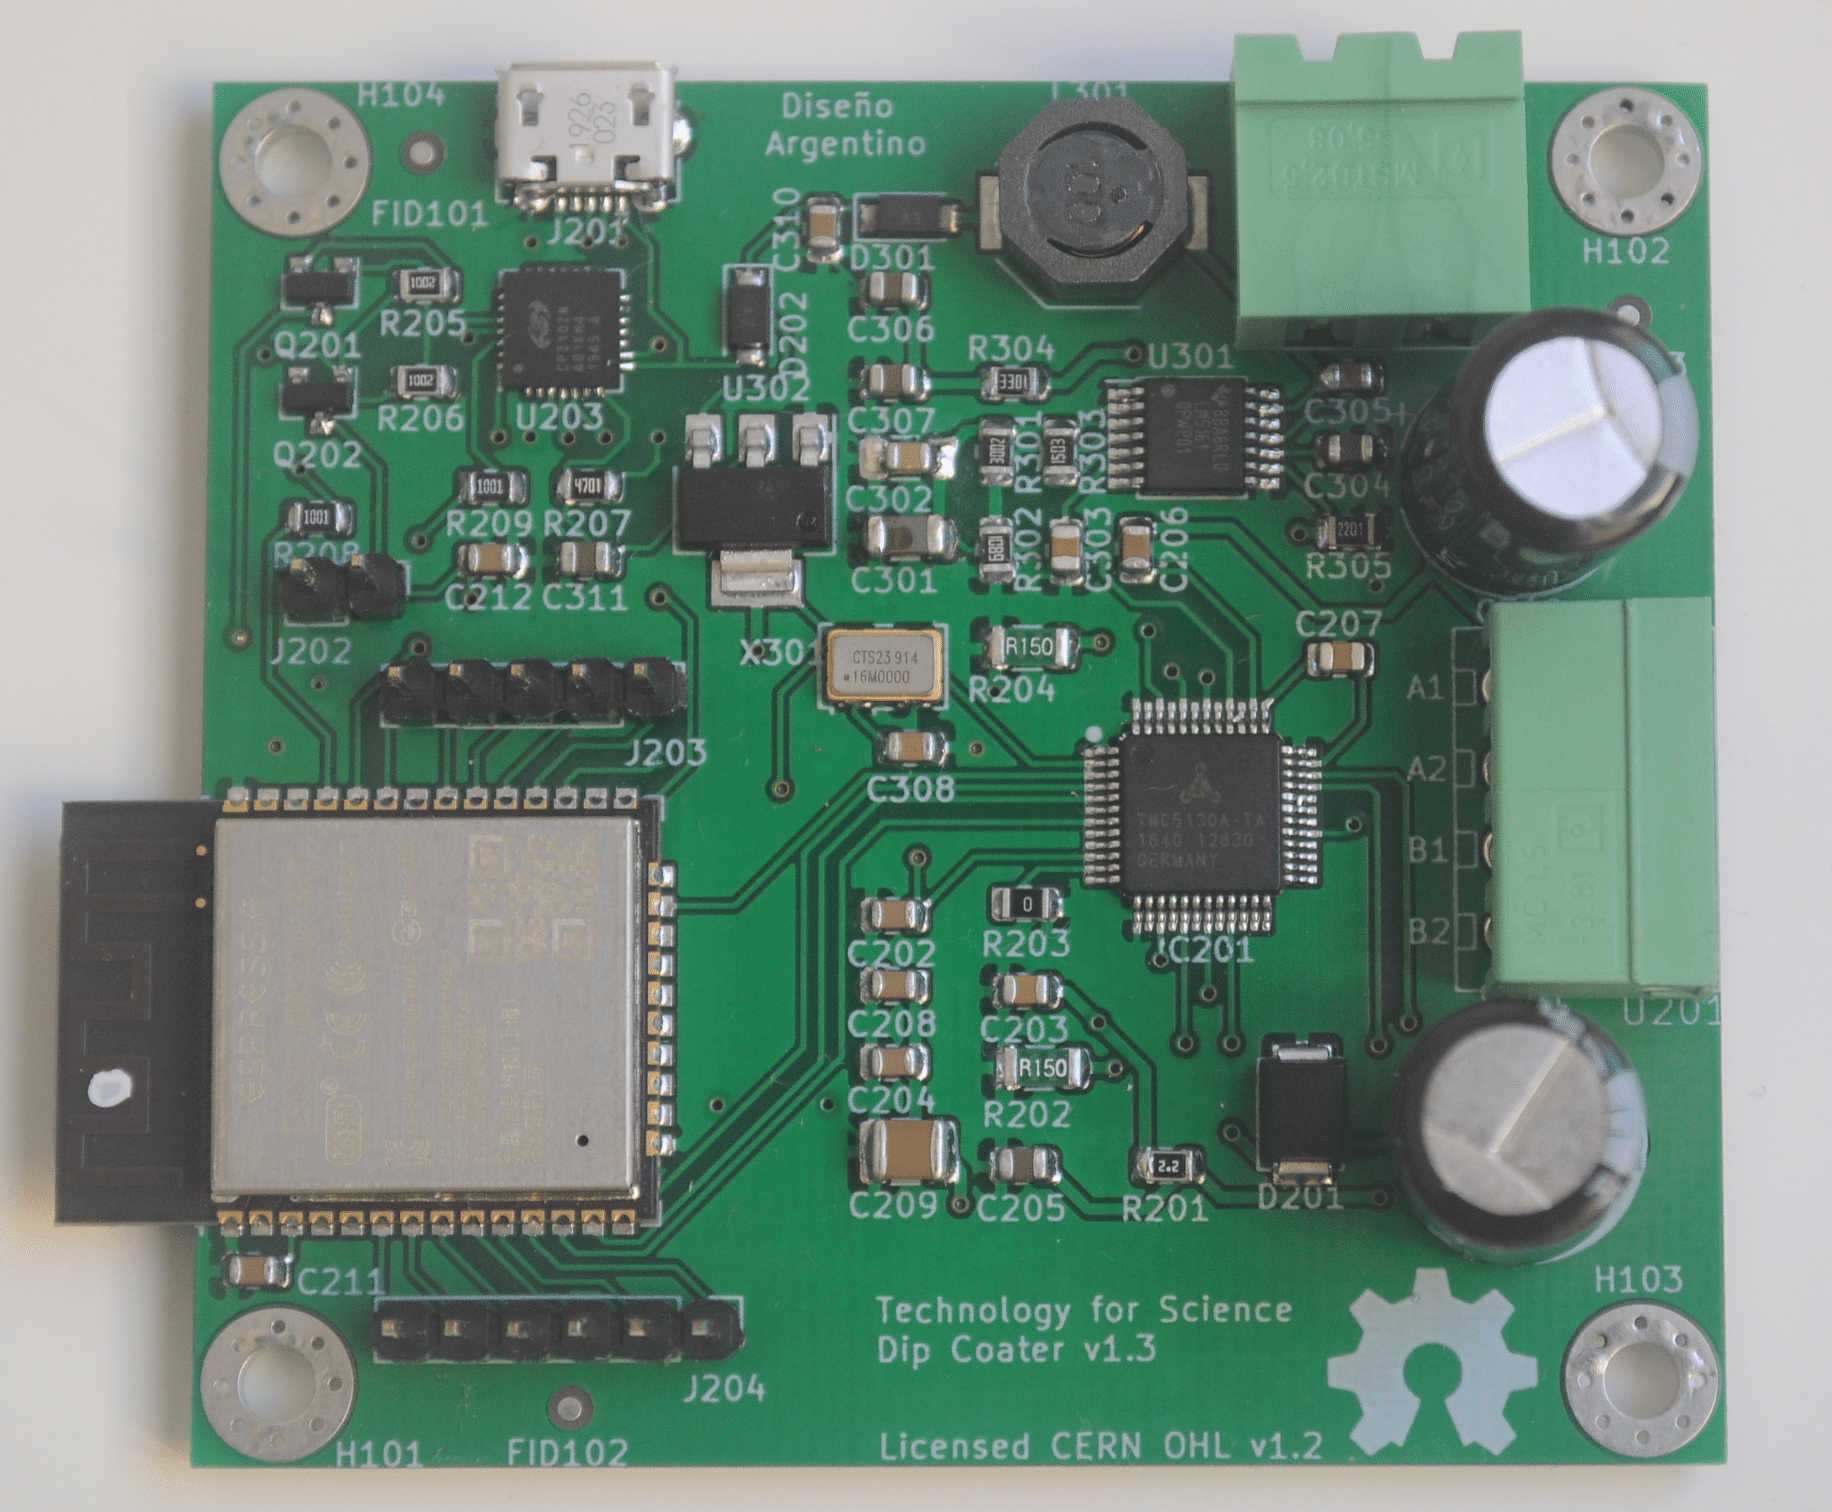
\includegraphics[width=1\textwidth]{./Figures/dip_real_model.pdf}
	\caption{Placa fabricada MAYER SRL.}
	\label{fig:dip_real_model}
\end{figure}

%----------------------------------------------------------------------------------------
%	SECTION 2
%----------------------------------------------------------------------------------------

\section{Firmware}

\subsection{Capas de abstracción}
\subsection{Framework de trabajo}
\subsection{Módulos principales}



%----------------------------------------------------------------------------------------
%	SECTION 3
%----------------------------------------------------------------------------------------

\section{Estructura mecánica}
\subsection{Fabricación de piezas personalizadas a través de mecanizado CNC}

Como se mencionó en la \ref{sec:estructura_mecanica} se utilizó para el diseño mecánico del equipo el software BOBCAD. El módulo CAD del software nos permite realizar un modelo 2D y 3D de pieza necesario para luego poder fabricarlo. El prototipo de dip coater cuenta actualmente con dos piezas mecanizadas. Podemos observar en la figura \ref{fig:carro} la pieza que se acopla al carro de la guiá lineal presentada en la sección \ref{sec:estructura_mecanica}.

\begin{figure}[ht]
	\centering
	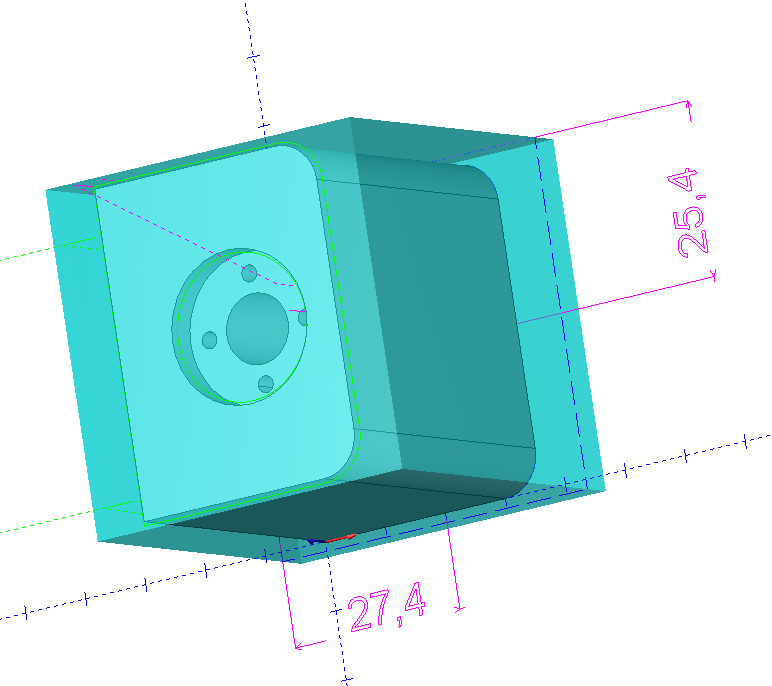
\includegraphics[width=.5\textwidth]{./Figures/3d_carro.png}
	\caption{Pieza personalizada para el carro.}
	\label{fig:carro}
\end{figure}

Y en la figura \ref{fig:estructura_superior} el soporte superior que sostiene el motor paso a pasos y el  tornillo que esta acoplado al eje del motor.

\begin{figure}[ht]
	\centering
	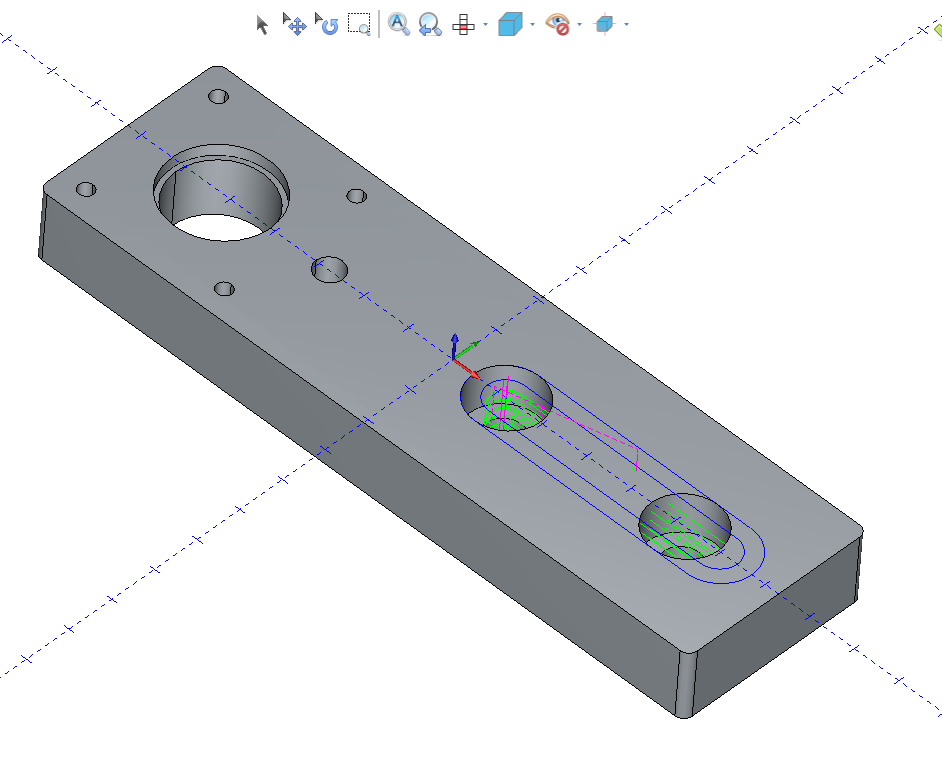
\includegraphics[width=.5\textwidth]{./Figures/3d_top.png}
	\caption{Piezas personalizado para sostener estructura superior.}
	\label{fig:estructura_superior}
\end{figure}

Primero se fabricaron las piezas a través de impresión 3D en plástico, luego que las piezas fueron probadas, testeadas y aprobadas en el prototipo se paso a la fabricación aluminio.
La estrategia utilizada en el mecanizado es por el método de arranque de viruta, es decir que se parte de un bloque de aluminio y las herramientas de corte van penetrando y desventando el bloque hasta lograr la pieza. Esta estrategia se programa en la parte CAM del software, se puede observar en la figura \ref{fig:estrategia}

\begin{figure}[ht]
	\centering
	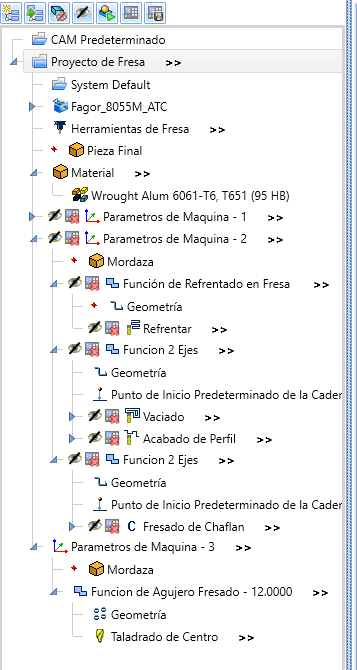
\includegraphics[width=.5\textwidth]{./Figures/3d_estrategia.png}
	\caption{Estrategias de mecanizado en software Bodcad.}
	\label{fig:estrategia}
\end{figure}



\subsection{Modelos 3D y real}

\begin{figure}[ht]
	\centering
	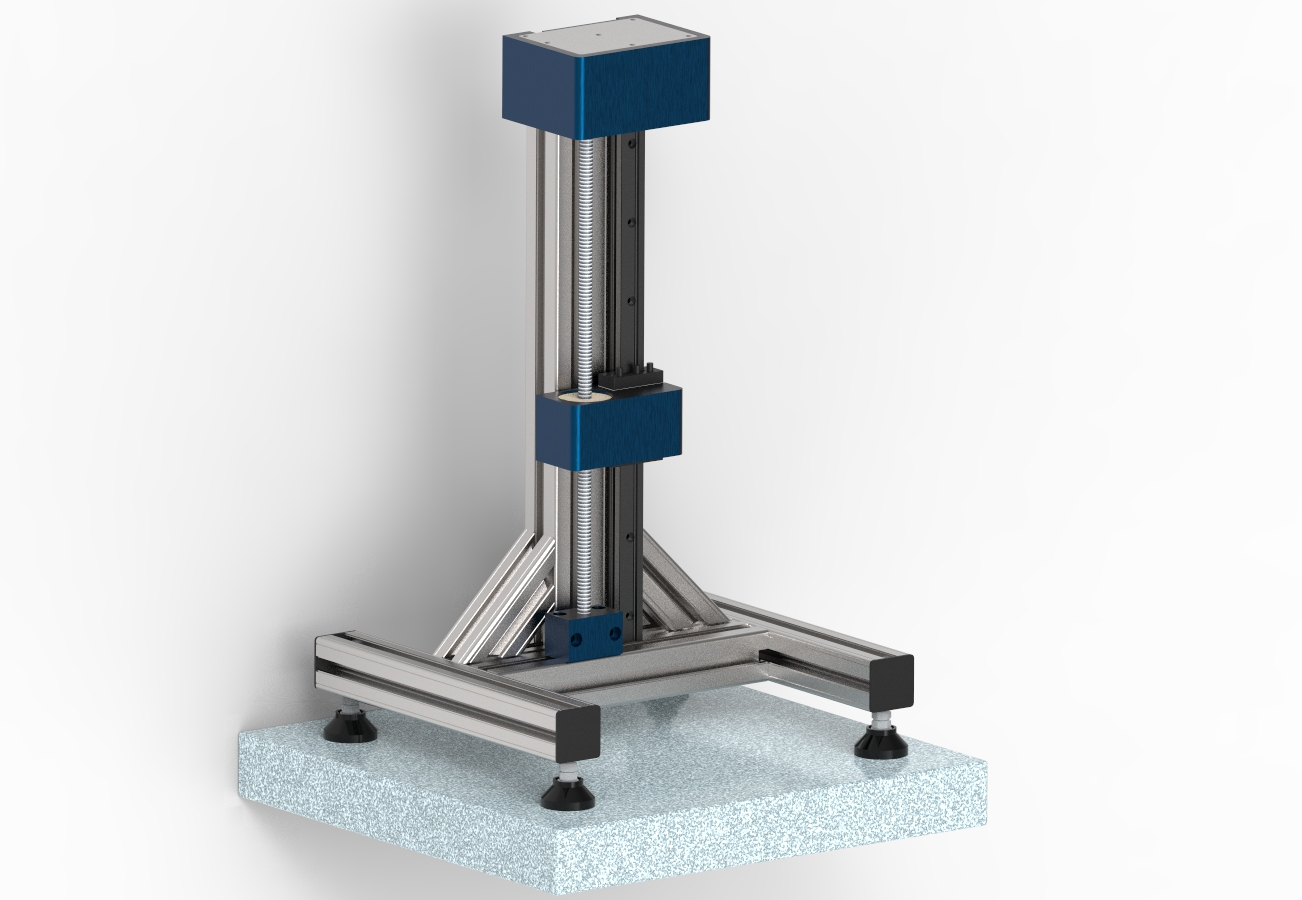
\includegraphics[width=.8\textwidth]{./Figures/3d.jpg}
	\caption{Modelo 3D.}
	\label{fig:mecanica_3d_model}
\end{figure}

\begin{figure}[ht]
	\centering
	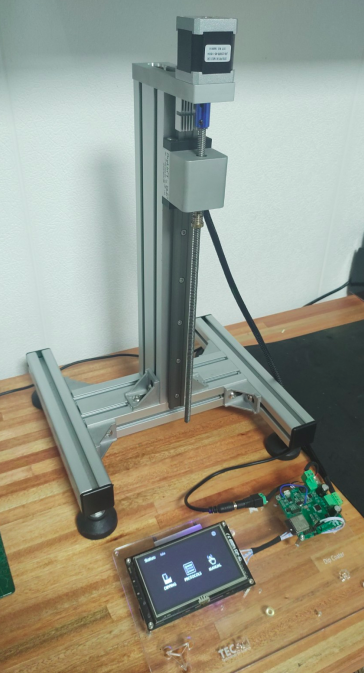
\includegraphics[width=.5\textwidth]{./Figures/real.png}
	\caption{Primer prototipo dip coater TECSCI.}
	\label{fig:mecanica_real_model}
\end{figure}